\documentclass[letter,doc,natbib,11pt]{apa7}  %% man <-> jou <-> doc

\usepackage[american]{babel}
\usepackage[utf8x]{inputenc}
\usepackage{amsmath}
\usepackage{graphicx}
\usepackage[colorinlistoftodos]{todonotes}
\usepackage{xcolor}


% use this for URLs
\usepackage{hyperref}
\hypersetup{
    colorlinks=true,
    citecolor=blue,
    linkcolor=blue,
    filecolor=blue,      
    urlcolor=blue,
}

% for cross references back to the main doc
% use \zref{} and \zlabel{} instead of latex native \ref{} and \label{}
\usepackage[xr, user, titleref]{zref}
\zexternaldocument{apa_ms}  % other .tex file to cross reference

% use this to include text files verbatim (not shown)
\usepackage{verbatim}

%use this package for highlighted source, e.g., research_report.tex
\usepackage{minted}
\setminted[latex]{
  frame=lines,
  bgcolor=bgc,
  fontsize=\footnotesize,
  linenos
}

% use this to include multipage pdf docs, e.g., conveted jupyter notebook, other docs
\usepackage{pdfpages}


\title{Supporting Information: Analyzing open science data in style: A reproducible repoducible research report report}
\shorttitle{Supporting Information: Reproducible reports with LaTeX{}}
\author{Thomas P. Urbach}
\affiliation{Kutas Lab \\ Cognitive Science Department \\ University of California, San Diego}

\begin{document}
\maketitle

\tableofcontents

\section{Summary}

Additional information can go here and be formatted to APA 6th
guidelines or something else. The supporting information and main
document can use the same research\_report.bib file so the references
match. With {\tt \textbackslash usepackage[xr,user,titleref]\{zref\}},
you can cross-reference back and forth between documents \ldots the
main report and this SI. For instance here is a reference to
Figure~\zref{ms:multipanel} in the main document. The reference is via the
label, i.e., {\tt \textbackslash zlabel\{ms:multipanel\}} so if the figure
is moved to a different page or its number changes because of
additions or deletions, this reference by number will update
automatically. The following sections show the source files that
generated the plots, figures, manuscript and supporting information pdfs.


APA 7th docs \url{http://ctan.math.washington.edu/tex-archive/macros/latex/contrib/apa7/apa7.pdf}
APA 6th docs \url{http://ctan.math.utah.edu/ctan/tex-archive/macros/latex/contrib/biblatex-contrib/biblatex-apa6/biblatex-apa6.pdf}




% For APA 7th TeXLive 2020 use change the figure captions from
% 
%   \caption{First sentence. Rest of the caption.}
% 
% to 
% 
%   \caption{First sentence.} \figurenote{Rest of caption.}
% 
% and this preamble
% 
% \documentclass[man,biblatex,10pt]{apa7}
% \usepackage{csquotes}
% \DeclareLanguageMapping{american}{american-apa}
% \usepackage[backend=biber,style=apa]{biblatex}



\section{System setup}

\subsection{Installing conda environments}

If you already use conda environments in a recent linux operating
system, you can install a minimal conda environment to run the
notebooks like so and follow the prompt (or omit -y to the end of the
command to install the packages without prompting).

\begin{minted}{bash}
conda create -n apa67_report pandas pyarrow matplotlib jupyter firefox -y
$ activate apa67_report
$ jupyter notebooks
\end{minted}

If you are not yet set up to use conda environments, you can follow
the instructions to download and install a minimal conda installer,
miniconda3
(\href{https://docs.conda.io/en/latest/miniconda.html}). This provides
just enough infrastructure to create a conda environemnt and install
packages as shown in the example above. If you want to create conda
environments and install packages faster, then install the `mamba`
conda package (\href{https://mamba.readthedocs.io/en/latest/}).

If you are not yet set up to use conda environments and don't want to
be then you are on your own. You can run pipeline\_1.ipynb if you have
numpy, pandas, matplotlib and jupyter.  You need the spudtr package to
run pipeline\_2.ipynb. Older versions are available via pip install,
but there is no assurance it is compatible with the versions of
packages you already have installed.

\subsection{Installing \LaTeX}

\subsubsection{Linux Installation via network}

You do not need to be root or admin to install TeX Live over the
networks and best practices are to install your copy in your
directory. That way you control the version and packages you
use. First read through the quick installation instructions
\href{https://www.tug.org/texlive/quickinstall.html}{here}. Then,
(summarizing from
\url{https://www.tug.org/texlive/acquire-netinstall.html}):

\begin{enumerate}

\item Download \url{install-tl-unx.tar.gz} to some scratch/working
  directory, unpack the archive, change to the new directory it
  made, i.e., \mbox{install\textendash tl\textendash YEARMONTHDAY} for
  whatever version, and run the installer.

  \begin{minted}{bash}
    $ tar -xf install-tl-unx.tar.gz 
    $ cd install-tl-20200814
    $ perl install-tl
  \end{minted}

  Follow the prompts, make sure you are happy with and have write
  permissions in the default installation directory, and press ``i''
  to install.

\item Update your ~/.bashrc file with the path to the new TeX Live
  installation.

  \begin{minted}{bash}
    PATH=/home/turbach/texlive/2020/bin/x86_64-linux:$PATH
    INFOPATH=/home/turbach/2020/texmf-dist/doc/info:$INFOPATH
    MANPATH=/home/turbach/2020/texmf-dist/doc/man:$MANPATH
  \end{minted}

\end{enumerate}

That's it, you have a complete functioning installation of \LaTeX{}
with the latest packages, TeX Live 2020 as of this writing.

The installation probably has everything you need including the apa6
and apa7 styles used for this report.

If there is a new package or update you want and you want to manage
the TeX packages with the TeX Live GUI you also need to install
perl/tk. There is a conda package for this, you can install into any
compatible conda env.

  \begin{minted}{bash}
    $ conda activate some_general_purpose_env
    $ conda install perl-tk -c BioBuilds -y
  \end{minted}


\subsubsection{OSX Installation}

See instructions for MacTeX here: \url{https://www.tug.org/mactex/}

\subsubsection{Windows}


See Quick Install instructions 
\href{https://www.tug.org/texlive/quickinstall.html}{here}

and Windows installer instructions
\href{https://www.tug.org/texlive/acquire-netinstall.html}{here}.


% The next two sections show the (converted-to-pdf)
% jupyter notebook for generating the figures, lateLaTeX{} .tex file for the main report and the jupyter
% notebook that generates the pdf plots for the filter figures.

%  ------------------------------------------------------------
% Jupyter notebook source
\newpage
\normalsize
\section{Source: author\_analysis.ipynb}\zlabel{si:analysis_nb}

The pdf of the notebook is generated by {\tt jupyter convert ... --to pdf}. The
LaTeX{} package {\tt pdfpages} is used to slurp it into the SI pdf.

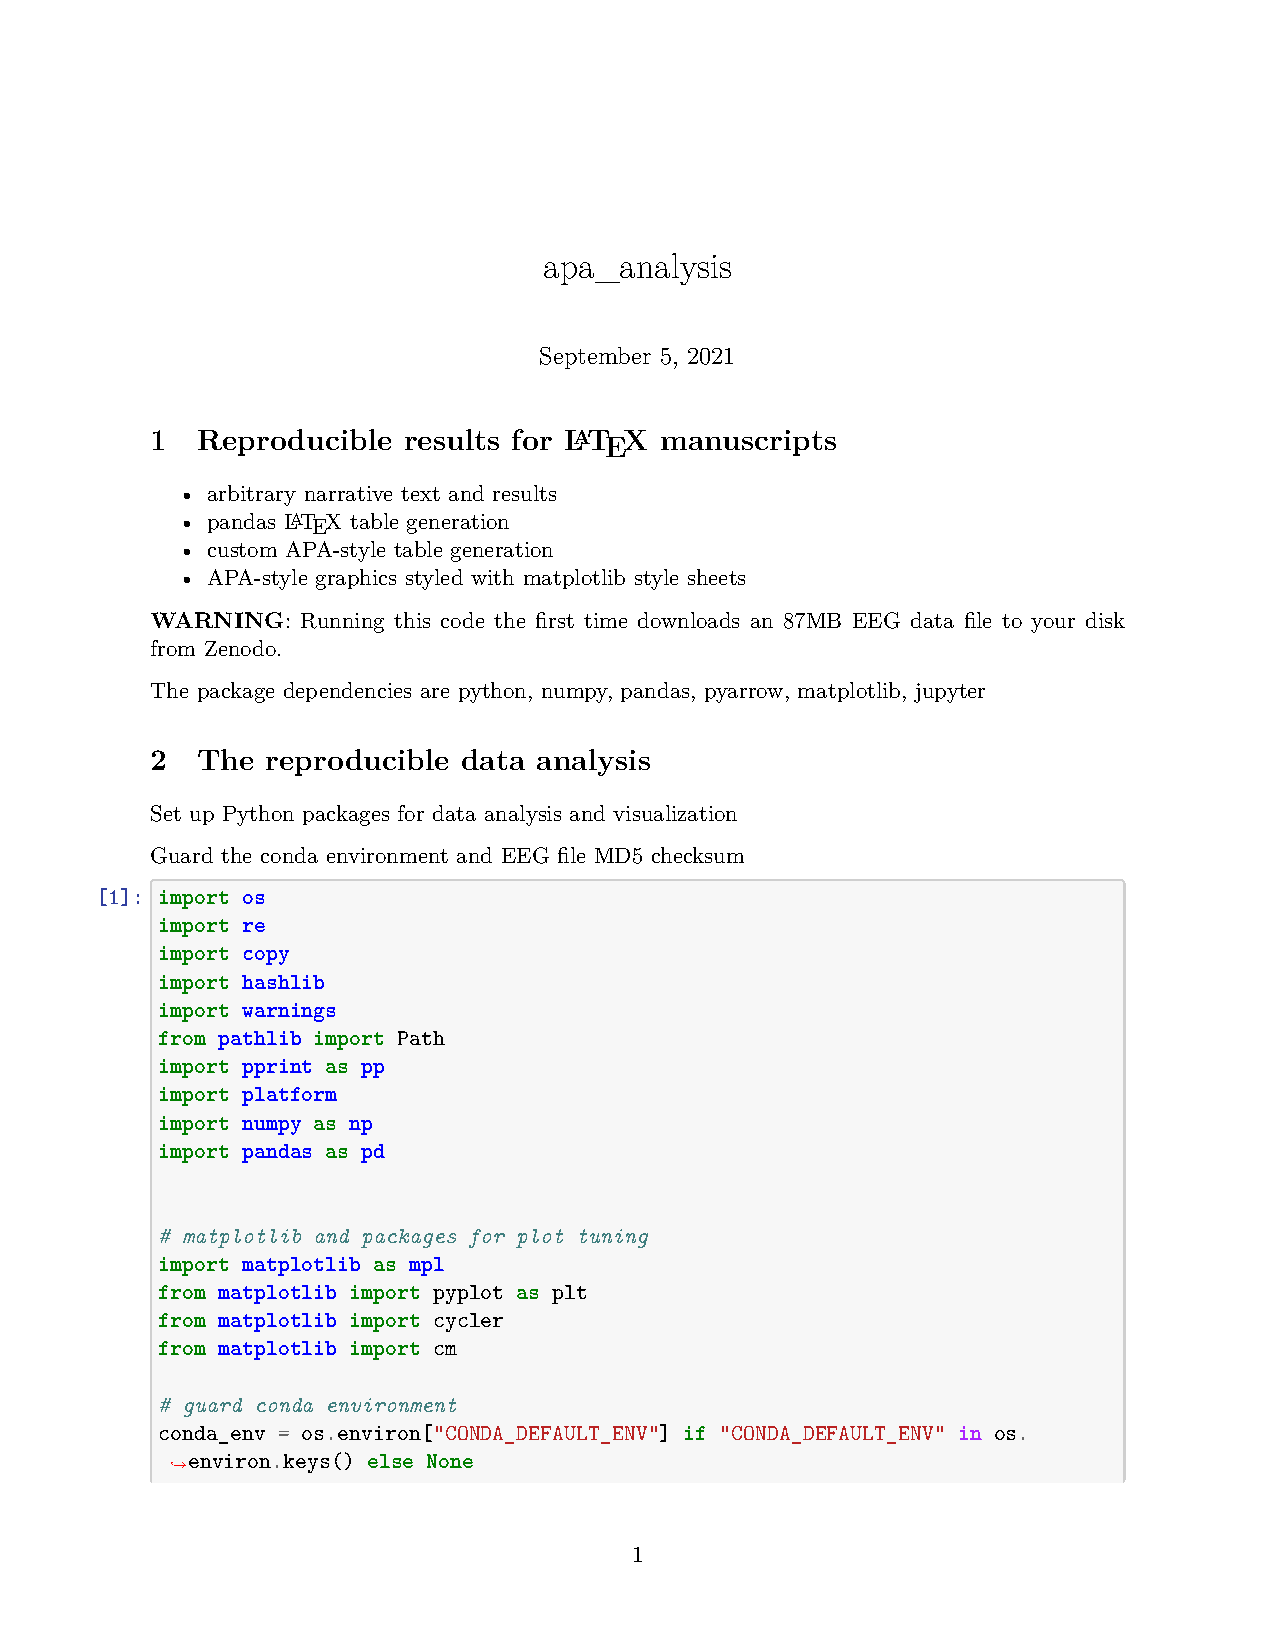
\includepdf[pages={1-}]{apa_analysis}


% ------------------------------------------------------------
% research report LaTeX
\newpage
\section{Source: {\tt research\_report.tex}}\zlabel{apa_ms_tex}
This is the LaTex{} for the main report. 

\definecolor{bgc}{rgb}{1.0,.96,1.0}
\inputminted{latex}{apa_ms.tex}


% ------------------------------------------------------------
% supporting information LaTeX
\newpage
\section{Source: {\tt author\_si.tex}}\zlabel{apa_si_tex}

This is the LaTex{} for this Supporting Information, i.e., it is 
typesetting itself. 

\inputminted{latex}{apa_si.tex}


% ------------------------------------------------------------
% Figure 1 LaTeX
\newpage
\section{Source: {\tt fig1.tex}}\zlabel{si:fig1_src}
This is basic LaTex{} template for a free-standing .tex file that pdflatex can turn
into a .pdf graphic for import or upload. It is just the graphic, no caption or numbering.

\inputminted{latex}{apa_fig1.tex}


% ------------------------------------------------------------
% Figure 2 LaTeX
\newpage
\section{Source: {\tt fig3.tex}}\zlabel{si:fig3_src}

This is the LaTex{} for the multipanel TikZ figure with fancy layout
and annotation stuff. Again, just for the pdf graphic, no caption.

\inputminted{latex}{apa_fig2.tex}

% ------------------------------------------------------------
% Makefile
\newpage
\section{Source: \mintinline{makefile}{Makefile}}\zlabel{si:makefile_src}
This is the Makefile used to build/rebuild the ms, si, figs indidually
and all the documents in one fell-swoop.

\inputminted{makefile}{Makefile}


% ------------------------------------------------------------
% bib
\newpage
\section{Source: {\tt research\_report.bib}}\zlabel{si:bib_src}
This is the .bib for citations and references, shared by the ms and this SI. 

\inputminted{bibtex}{apa_ms.bib}

% Supporting Information References (if any)
\bibliography{research_report}

\end{document}
